\documentclass[10pt]{article}
\usepackage[T1]{fontenc}
\usepackage{lmodern}
\usepackage[margin=1in]{geometry}
\usepackage{amsmath,amssymb,booktabs,graphicx,array}
\usepackage[colorlinks=true,linkcolor=blue,urlcolor=blue,citecolor=blue]{hyperref}
\title{Reducing TRIBE v2 Feature-Extraction Cost\newline with Numerical and Prediction Regression Checks}
\author{}
\date{November 8, 2026}
\begin{document}
\maketitle
\begin{abstract}
TRIBE v2 extracts video, audio, and contextual language representations before
predicting brain responses. We optimize this extraction stage without retraining,
changing checkpoints, or reducing input resolution. The video path removes an
unused predictor, reduces selected hidden states as they are produced, and
reuses preprocessed frames at identical timestamps. The text path transfers only the
tokens and layers needed for each target word and disables an unused key--value
cache. The audio path selects output timestamps before transferring features
to the CPU. We compare uncached extraction against neuralset 0.0.2 on an AMD
Radeon RX 9070 XT, with fixed inputs, batch composition, and model dtypes.
The FP32 video rewrite is 1.23 times faster on the stated short-event workload;
text and audio are 2.27 and 1.14 times faster with bitwise-equal sampled outputs.
The final FP16 video path with CPU prefetch is 12.07 times faster than the
original FP32 path and reduces peak tensor allocation by 76.16\%. A separate
60-second comparison isolates prefetch: 7.42\% shorter median time and
bitwise-identical sampled FP16 features across three paired repetitions. The
FP16 precision change meets prespecified prediction-regression margins in all
672 comparisons across 168 existing subjects and four movies. These checks do not establish accuracy equivalence on unseen stimuli
or on an independently held-out population.
\end{abstract}

\section{Problem and baseline}
The reported bottleneck in the evaluated TRIBE v2 workflow is stimulus feature extraction,
not the subsequent brain encoder. This report therefore evaluates fresh extraction
from local videos, audio, and existing word contexts. Transcription and the brain
encoder are outside the extraction timings. A separate companion report documents
an optional affine readout optimization; its millisecond timings must not be
interpreted as video-processing throughput.

We fix the upstream TRIBE v2 source at
\texttt{af58661791a35} and use the installed neuralset
0.0.2 extraction code as the reference~\cite{tribe,neuralset}. Its relevant source files were checked
against the published 0.0.2 wheel. The released configuration uses
\texttt{facebook/vjepa2-vitg-fpc64-256}, \texttt{facebook/w2v-bert-2.0}, and
\texttt{meta-llama/Llama-3.2-3B}. The float32 video/audio and bfloat16 text
rewrites preserve their weights, preprocessing, time
sampling, and layer aggregation. Video and audio run in float32; the tested
Transformers loader chooses bfloat16 for Llama. The language comparison preserves
that baseline dtype rather than silently promoting or quantizing it.
We separately evaluate an opt-in video float16 configuration, retaining float32
token means and the original 64-frame input. Its accuracy comparison uses
downstream brain predictions rather than requiring identical feature values.

\section{Changes and invariants}
\subsection{Video: retain summaries, not all token states}
Each output time uses 64 frames from a four-second causal window, at an output
rate of 2 Hz. The Hugging Face V-JEPA 2 implementation provides encoder hidden
states and also runs a predictor by default~\cite{vjepa,hfvideo}. Neuralset consumes only the encoder
hidden states. We remove the predictor before moving weights to the GPU.
This removes 22,381,312 of 1,034,555,264 loaded parameters; it does not compress
the encoder or reduce the original checkpoint's download size.

Let $H_\ell\in\mathbb{R}^{N\times D}$ be one encoder hidden state, with $N$ tokens
and $D$ channels. The cached feature for a selected layer is
\begin{equation}
z_\ell=\frac{1}{N}\sum_{i=1}^{N}H_{\ell,i,:}.
\end{equation}
The reference materializes all hidden states, selects layers, then averages
tokens. We compute each selected $z_\ell$ immediately and release the preceding
full token state as the next layer runs. All encoder layers and their attention
operations remain. For the tested checkpoint, $N=8192$ and $D=1408$.
The hidden-state tuple contains the embedding output followed by 40 layer
outputs; its last element precedes the encoder's final layer normalization.
Applying that normalization here would change the representation.

Layer selection still uses the reference's rounded, evenly spaced 20 indices.
This is algebraically the same mean, although different reduction layouts can
change floating-point rounding. We therefore check numerical error separately.
The frame cache retains only the current window and reuses frames at exactly
equal floating-point timestamps. It neither rounds timestamps nor changes
clamping at event boundaries. It caches processed CPU tensors, so both decoding
and preprocessing are avoided for repeated timestamps. In a separate input
check, ten windows per movie requested 640 frames but only 81 unique timestamps;
the resulting processed inputs were bitwise identical. The tested videos have
fixed frame dimensions and use no optional preliminary image-size limit.
Variable-resolution videos with that optional limit are outside this check.
The final implementation prepares one upcoming CPU frame window on a worker
while the current window runs on the GPU. It consumes each future in timestamp
order and retains at most one pending window. An executor context inside the
reader cleanup block joins outstanding work before closing the video, including
on inference errors. This adds bounded CPU lookahead storage; host-memory
reduction is not claimed.

\subsection{Text: select before transfer}
The reference transfers hidden states for every layer and every token to the
CPU before isolating a target word. We keep the same tokenizer, context strings,
padding, truncation, batch size, and target-token bounds, but transfer only the
selected layers and target tokens. Token averaging still occurs on the CPU in
the original dtype, followed by conversion to float32. The model's unused
generation cache is disabled. We retain the reference's EOS/padding convention
and truncation behavior, even where a different convention might be preferable
for a new experiment: this is a regression-preserving implementation change.

\subsection{Audio: select timestamps before transfer}
The Wav2Vec2-BERT~\cite{hfaudio} audio reference transfers every native-rate hidden state and then uses nearest
interpolation on the CPU to reach 2 Hz. We apply the same nearest interpolation
to each hidden state on the GPU and transfer the smaller result. Target length
comes from the event duration and the original \texttt{Frequency.to\_ind} rule.
The audio reference retains all 25 layers despite \texttt{cache\_n\_layers=20};
we preserve this behavior. Selecting 20 layers here would alter the subsequent
layer groups and invalidate the comparison.
Native-rate GPU hidden states are released before starting the next event.

All variants use distinct extractor class names and cache namespaces. Existing
feature caches and default extractors remain available. The optimized paths
target the released configuration; they reject unsupported modes explicitly.

\section{Evaluation protocol}
We bypass Exca's automatic feature cache in both conditions and execute actual
extraction. Video samples are four independent four-second events, one per movie,
with offsets 120, 300, 480, and 660 seconds. This gives 32 model inputs per pass.
The first windows clamp to the beginning of each sampled event exactly as in
the reference. They are not represented as the corresponding full-movie features.
Text samples cover word positions 100--115 and 800--815 from each movie, preserving
four-word batches and existing contexts: 128 words in total. Audio samples use
four 60-second events. These are local HCP stimulus inputs; neither stimuli,
transcripts, subject data, nor extracted arrays are redistributed.

For the FP32 video rewrite, BF16 text rewrite, and FP32 audio rewrite, we require
finite outputs, equal shapes and timing metadata, and the elementwise gate
\begin{equation}
|\widehat{x}-x|\leq10^{-5}+10^{-4}|x|,
\end{equation}
where $x$ is the original feature. This is a numerical regression criterion,
not a margin for fMRI prediction accuracy. The separate FP16 video candidate
may fail this feature gate; its acceptance instead requires every downstream
subject/movie comparison to meet the score margins below. We also report bitwise equality,
maximum absolute error, and failed-element counts. Tolerances are fixed before
the final comparison and are not relaxed for a faster candidate.

The benchmark records condition order, individual wall times, initialization
scope, and peak PyTorch tensor allocation. GPU work is serialized. Peak allocation
is not total physical VRAM. Small numbers of repeated workloads describe this
machine and sample set; they do not provide population confidence intervals.

\subsection{Prediction checks across existing subjects}
The first comparison uses one existing subject to check the full four-movie
pipeline. An inventory conducted before the candidate scores identified 168
subjects with all four BOLD caches. We therefore also compare the unchanged
original and candidate average-subject predictions against every one of those
672 subject/movie pairs. This does not repeat feature extraction per subject.

For each pair, the absolute mean parcel-correlation change must be at most
$10^{-4}$, the maximum absolute change over 360 parcel correlations at most
$10^{-3}$, and the absolute relative labeled-vertex MSE change at most $10^{-3}$.
These are the same margins fixed for the initial subject; they are not adjusted
for the cohort. We preserve lag $-5$, trim each movie to its original valid
length, and use the same canonical scoring implementation. A failed pair
precludes acceptance. Public cohort results contain movie aggregates, extrema,
and quantiles; participant identities and individual diagnostics stay private.
The subjects are existing cached inputs, not a newly held-out population, and
no statistical equivalence test is claimed.

\section{Measured results}
The first four conditions describe the stages before CPU prefetch was added to video extraction. They were measured on the AMD RX~9070~XT. Video times include model loading; text and audio times exclude loading. The samples contain 32 video clips, 128 words, and four 60-second audio events. Each modality is a separate workload; these speed ratios do not measure a combined pipeline. Table~\ref{tab:features-performance} reports medians and ratios; Table~\ref{tab:features-raw} retains both repetitions. No confidence intervals are claimed.

\begin{table}[htbp]\centering\sffamily\small
\caption{Before video prefetch: median extraction time and peak GPU tensor allocation across two repetitions per condition. Speedup is original/candidate median; peak allocation is the maximum across repetitions. Video times include load; text and audio exclude load. *Video FP16 uses a separately recorded FP32 video baseline and is not interleaved with the FP16 runs.}\label{tab:features-performance}
\begin{tabular}{@{}lrrrrr@{}}\toprule
Condition & Orig. (s) & New (s) & Speedup & Orig. (GiB) & New (GiB) \\\midrule
Video FP32 & 242.102 & 197.060 & 1.23 & 9.468 & 4.517 \\
Video FP16* & 242.102 & 21.182 & 11.43 & 9.468 & 2.257 \\
Text BF16 & 14.265 & 6.289 & 2.27 & 7.530 & 7.039 \\
Audio FP32 & 4.638 & 4.085 & 1.14 & 7.464 & 7.464 \\
\bottomrule\end{tabular}\end{table}

\begin{table}[htbp]\centering\sffamily\small
\caption{Before video prefetch: raw extraction times (s). Video FP32 and FP16 are not interleaved; the FP16 candidate is compared against the separately recorded FP32 baseline median.}\label{tab:features-raw}
\begin{tabular}{@{}lrr@{}}\toprule
Condition & Original repetitions (s) & Candidate repetitions (s) \\\midrule
Video FP32 & 241.809, 242.395 & 197.043, 197.076 \\
Text BF16 & 13.049, 15.481 & 6.269, 6.308 \\
Audio FP32 & 4.670, 4.605 & 4.081, 4.090 \\
Video FP16* & 241.809, 242.395 & 21.358, 21.006 \\
\bottomrule\end{tabular}\end{table}

Figure~\ref{fig:features-performance} shows normalized extraction time with the original as 1 and the peak GPU tensor allocation. Candidate repetitions appear as points. FP16 changes feature values, so downstream score margins determine its acceptance.

Figure~\ref{fig:features-accuracy} reports score drift over all 168 existing subjects. The worst subject/movie pair determines acceptance; averaging subjects cannot hide a failure. The initial single-subject alignment check is retained in Table~\ref{tab:features-accuracy}.

\begin{table}[htbp]\centering\sffamily\small
\caption{Existing-subject brain-score agreement for the FP16 video path. Baseline and candidate mean parcel correlations are shown to six decimals; deltas use scientific notation. Margins: mean $|\Delta r| \leq 10^{-4}$, max parcel $|\Delta r| \leq 10^{-3}$, $|\Delta \mathrm{MSE}|/\mathrm{MSE} \leq 10^{-3}$.}\label{tab:features-accuracy}
\begin{tabular}{@{}lrrrrr@{}}\toprule
Movie & Orig. mean $r$ & New mean $r$ & $\Delta$ mean $r$ & Max $|\Delta r|$ & Rel. MSE \\\midrule
Movie 1 & 0.236518 & 0.236493 & $-2.49\times10^{-5}$ & $3.80\times10^{-4}$ & $1.62\times10^{-6}$ \\
Movie 2 & 0.263297 & 0.263328 & $3.15\times10^{-5}$ & $2.74\times10^{-4}$ & $-8.88\times10^{-6}$ \\
Movie 3 & 0.200522 & 0.200527 & $4.67\times10^{-6}$ & $3.81\times10^{-4}$ & $-3.67\times10^{-6}$ \\
Movie 4 & 0.257067 & 0.257074 & $6.19\times10^{-6}$ & $2.87\times10^{-4}$ & $-5.39\times10^{-6}$ \\
\bottomrule\end{tabular}\end{table}

4 of four movies satisfy all three prespecified margins. These are engineering margins, not statistical equivalence tests.

\begin{table}[htbp]\centering\sffamily\small
\caption{FP16 regression across all 168 existing subjects per movie. Worst changes take the maximum absolute change across subjects (and parcels for parcel r); each subject/movie pair uses the fixed margins.}\label{tab:cohort}
\begin{tabular}{@{}lrrrrr@{}}\toprule
Movie & Orig. mean $r$ & New mean $r$ & Max $|\Delta\bar r|$ & Max $|\Delta r|$ & Max rel. $|\Delta$MSE$|$ \\\midrule
1 & 0.207309 & 0.207298 & $6.51\times10^{-5}$ & $7.08\times10^{-4}$ & $2.21\times10^{-5}$ \\
2 & 0.227327 & 0.227322 & $6.32\times10^{-5}$ & $4.21\times10^{-4}$ & $1.65\times10^{-5}$ \\
3 & 0.207018 & 0.207009 & $5.46\times10^{-5}$ & $7.88\times10^{-4}$ & $3.19\times10^{-5}$ \\
4 & 0.240679 & 0.240680 & $3.25\times10^{-5}$ & $4.23\times10^{-4}$ & $1.58\times10^{-5}$ \\
\bottomrule\end{tabular}\end{table}

Table~\ref{tab:cohort} covers all 672 subject/movie pairs; 0 exceed at least one margin. The cohort is an existing cache, not an independently held-out population. No participant identifiers or individual diagnostic rows are redistributed.

\begin{figure}[htbp]\centering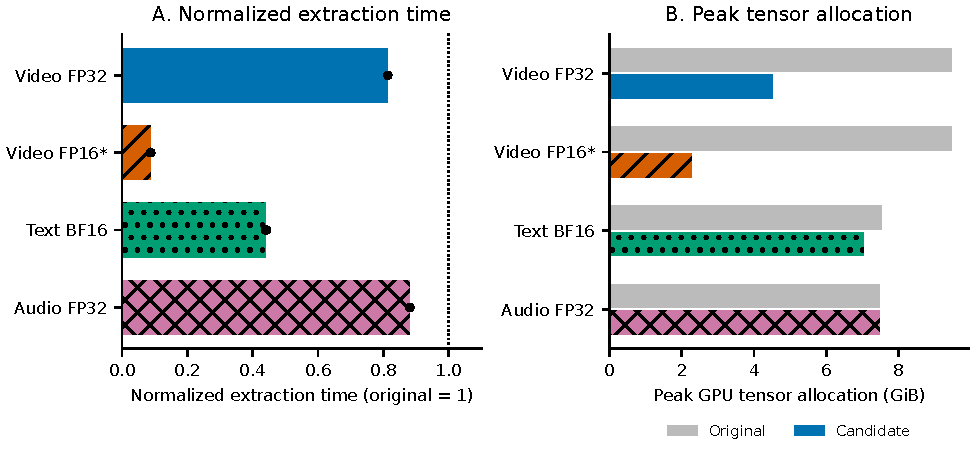
\includegraphics[width=\linewidth]{features-performance.pdf}\caption{Extraction costs before video prefetch. Left: bars show candidate/original median time; black points show the two candidate repetitions divided by the original median. Right: gray and colored bars show original and candidate peak GPU tensor allocation, respectively, taking the maximum of two runs. Video FP16 (*) was timed separately from the original FP32 runs. Allocation excludes non-PyTorch VRAM.}\label{fig:features-performance}\end{figure}

\begin{figure}[htbp]\centering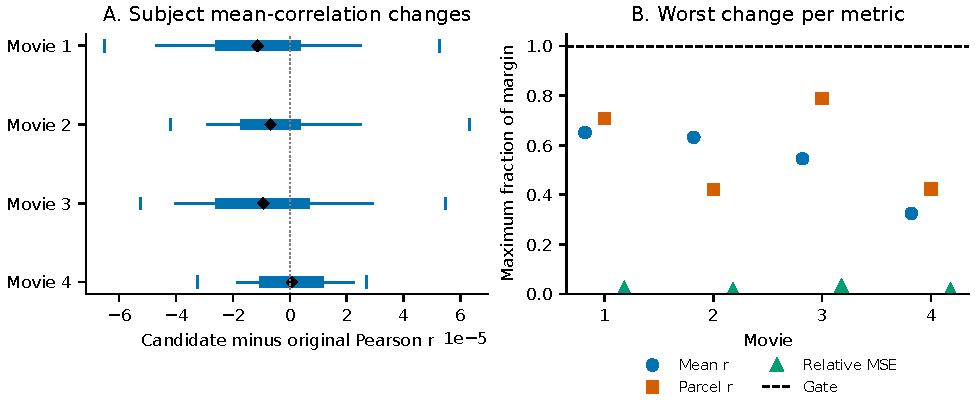
\includegraphics[width=\linewidth]{features-accuracy.pdf}\caption{Serial float16 video regression on four movies across 168 existing subjects. Left: diamonds, subject median change in mean parcel r; thick lines, interquartile range; thin lines, 5th--95th percentiles; ticks, extrema. These are subject distributions, not confidence intervals. Right: the maximum for each metric divided by its fixed margin; these maxima may come from different subjects. Circles show mean r, squares maximum parcel r, and triangles relative labeled-vertex MSE. Values at or below 1 pass.}\label{fig:features-accuracy}\end{figure}

\subsection{Final video path with CPU prefetch}

The final path overlaps one CPU frame window with GPU inference. Table~\ref{tab:prefetch-long} compares it with serial FP16 on one 60-second event. All three pairs are finite and bitwise equal over 3,379,200 values per pair. The 168-subject precision evaluation used the serial FP16 path; the full cohort was not re-extracted with prefetch. The separate prefetch check covers these 120 clips.

\begin{table}[htbp]\centering\sffamily\small
\caption{Production prefetch: three alternating pairs on one 60-second event; loading included. Serial control performs the same CPU reads when the main thread requests each result.}\label{tab:prefetch-long}
\begin{tabular}{@{}lrr@{}}\toprule
Pair & Serial FP16 (s) & Prefetch FP16 (s) \\\midrule
1 & 74.334 & 69.814 \\
2 & 75.736 & 69.899 \\
3 & 75.503 & 70.282 \\
Median & 75.503 & 69.899 \\
\bottomrule\end{tabular}\end{table}

The median reduction is 7.42\%. One future bounds CPU lookahead to one window; GPU inference stays on the main thread. The worker is joined before the video reader closes, including on inference errors.

\begin{table}[htbp]\centering\sffamily\small
\caption{Final short-event extraction: 32 clips, two repetitions, model loading included. The original FP32 baseline was recorded separately; these conditions were not interleaved.}\label{tab:prefetch-short}
\begin{tabular}{@{}lrrr@{}}\toprule
Condition & Median (s) & Speedup & Peak (GiB) \\\midrule
Original FP32 & 242.102 & 1.00 & 9.468 \\
FP16 with prefetch & 20.051 & 12.07 & 2.257 \\
\bottomrule\end{tabular}\end{table}

The final short-event repetitions took 19.995, 20.106 s. The short-event and 60-second workloads differ; their speed ratios are not multiplied.


\section{Candidate decisions and scope}
Changing precision is a different intervention from removing unused work.
An exploratory float16 video run was much faster, but failed the feature gate.
We therefore evaluate it separately against frozen brain-score margins instead
of describing its features as numerically equivalent. Reusing common causal prefixes
across language contexts also changed outputs when sequence and batch shapes
changed; both bfloat16 and float32 probes failed the fixed gate. We retain the
original batch composition. A separately compiled video encoder passed a
single-input numerical probe, but its small observed steady-state gain and
additional compiler/version dependence do not justify a production default.

A 32-frame candidate failed the prespecified first-movie rejection screen.
Its mean parcel correlation increased by $2.23\times10^{-3}$, while individual
parcel changes ranged from $-4.19\times10^{-2}$ to $+3.61\times10^{-2}$.
Thus its aggregate improvement did not preserve regional prediction accuracy.
We retain 64 frames and do not infer a general failure of reduced-frame models
from this one-subject, one-movie screen. No additional subjects or movies were
used to accept the 32-frame configuration.

The float32 implementation changes preserve the learned representation in real
arithmetic; their floating-point agreement is tested on the stated inputs.
The separate float16 path is an approximate numerical implementation. No model was
pruned, distilled, retrained, or substituted. These results do not establish
accuracy equivalence across populations or unseen stimuli, nor do they include
ASR runtime. Further changes to precision or representations require a separate prediction
regression check for this workflow. Generalization claims require additional
held-out stimuli and subjects. The tested candidates and reviews are
resolved; this is not a proof that no future optimization is possible.

\section{Reproduction and review}
The repository contains the extractors, focused unit tests, public benchmark
scripts, aggregate JSON measurements, and this TeX source. The benchmark accepts
local event tables and writes no private stimulus paths or text into the public
result. Optional saved feature arrays are private inputs for downstream checks.
Model loading uses the user's existing Hugging Face access and model cache.
The executed comparisons used the same local cache in offline mode. Feature
loaders request model names without explicit revisions; the recorded video
revision comes from the cache spot check, and audio/text revisions describe
separately resolved configurations. These records do not pin all weight and
processor snapshots for future downloads. Exact reproduction is consequently
limited to the evaluated local snapshots and runtime.

DeepSeek V4.1 Flash produced implementation drafts through OpenCode Go. Codex
reviewed and corrected the changes, executed measurements, and obtained a
separate source review. Ninety tests passed in each of two Torch environments;
eight final report checks also passed, including five newly added tests. A fresh
four-second public prediction call exercised all three extractors and returned
finite predictions of shape $(4,20484)$ using existing word contexts. The review log distinguishes accepted findings from
claims rejected after checking the source. The upstream CC-BY-NC-4.0 license
and attribution remain in place.

\section{Recorded settings}
Tables~\ref{tab:feature-settings}--\ref{tab:score-settings} summarize the executed
conditions. There is no optimizer, learning rate, training split, or training
stopping rule: this study does not train weights. The stimulus samples are
engineering regression inputs, and no independent confirmatory population was
introduced for the existing 168-subject cache. Private paths and participant identifiers are omitted.

\begin{table}[htbp]\centering\sffamily\small
\caption{Feature-extraction settings and verification sources}
\label{tab:feature-settings}
\begin{tabular}{@{}>{\raggedright\arraybackslash}p{.21\linewidth}>{\raggedright\arraybackslash}p{.49\linewidth}>{\raggedright\arraybackslash}p{.24\linewidth}@{}}\toprule
Item & Executed value & Source \\\midrule
Video encoder & V-JEPA 2 ViT-g; 40 layers; width 1408; 64 frames; 256-pixel crop & Loaded model/config \\
Video outputs & 2 Hz; 4-second causal window; mean tokens; 20 cached states & Checkpoint config; extractor \\
Video precision & Reference/rewrite FP32; separate candidate FP16 with FP32 token means & Extractor; result JSON \\
Audio encoder & Wav2Vec2-BERT 2.0; width 1024; FP32; 16 kHz input; 2 Hz output & Model and extractor \\
Audio preprocessing & Original normalization and nearest interpolation; all 25 states retained & Neuralset; regression tests \\
Text encoder & Llama-3.2-3B; width 3072; BF16; four words per batch; 20 cached states & Loaded model; benchmark \\
Text contexts & Existing word contexts; context transform maximum length 1024; original tokenizer truncation & Events pipeline; benchmark \\
Layer groups & Original group means with boundaries 0.5, 0.75, 1.0 & Released checkpoint config \\
Feature gate & $|\widehat{x}-x|\leq10^{-5}+10^{-4}|x|$; finite values; identical shape and timing & Benchmark implementation \\
Video samples & Four 4-second events; offsets 120/300/480/660 s; 32 clips total. Prefetch pairs: one 60-s event at 120 s (120 clips) & Selection in result JSON \\
Text/audio samples & 128 words (two 16-word blocks/movie); four 60-second audio events & Selection in result JSON \\
Timing & Two short-workload repetitions/condition; alternating original/rewrite order; FP16 timed separately; three paired 60-s prefetch comparisons & Recorded run order \\
Timing scope & Cache bypassed; video includes model load; text/audio exclude model load; ASR excluded & Benchmark implementation \\
\bottomrule\end{tabular}\end{table}

\begin{table}[htbp]\centering\sffamily\small
\caption{Runtime and source revisions}
\label{tab:runtime-settings}
\begin{tabular}{@{}>{\raggedright\arraybackslash}p{.21\linewidth}>{\raggedright\arraybackslash}p{.49\linewidth}>{\raggedright\arraybackslash}p{.24\linewidth}@{}}\toprule
Item & Executed value & Source \\\midrule
Hardware & AMD Radeon RX 9070 XT, 16 GiB; Intel Core i5-13500 & Local runtime inventory \\
Software & Python 3.12.15; Torch 2.12.0+rocm7.14.0; HIP 7.14.60850; torchvision 0.27.0+rocm7.14.0 & Installed runtime \\
Dependencies & Transformers 5.14.1; neuralset/neuraltrain 0.0.2; Exca 0.5.20 & Installed runtime \\
CPU threads & OMP\_NUM\_THREADS=4; MKL\_NUM\_THREADS=4 & Launch environment \\
Compatibility & CPU Torch 2.6.0 with shared non-Torch dependencies; no clean-install claim & Separate test environment \\
Upstream TRIBE & \texttt{af58661791a35} & Git base revision \\
Implementation & \texttt{94ace50}: full 64-frame run; \texttt{63d759b}: audio lifetime and validation; \texttt{932e7fb}: cohort checks; \texttt{2ea6ccb}: prefetch & Local Git revisions \\
Brain checkpoint & \texttt{f894e78302094} & Local Hub snapshot \\
Video revision & \texttt{875c192b7b704} & Loaded model in cache spot check \\
Audio config revision & \texttt{da985ba0987f7} & Separately resolved config \\
Text config revision & \texttt{13afe5124825b} & Separately resolved config \\
\bottomrule\end{tabular}\end{table}

\begin{table}[htbp]\centering\sffamily\small
\caption{Approximate-video prediction regression protocol}
\label{tab:score-settings}
\begin{tabular}{@{}>{\raggedright\arraybackslash}p{.21\linewidth}>{\raggedright\arraybackslash}p{.49\linewidth}>{\raggedright\arraybackslash}p{.24\linewidth}@{}}\toprule
Item & Executed value & Source \\\midrule
Evaluation scope & Initial one-subject check; then 168 existing subjects, four HCP movies (672 pairs); no retraining; video alone replaced & Evaluation scripts and cache inventory \\
Original event grid & 15 events/movie; 60 total; original offsets/durations, including unequal tails & Original event table \\
Readout inputs & 40 windows of 100 s; video shape $(1,2,1408,200)$; unchanged text/audio & Frozen batches and metadata \\
Alignment check & All 40 original cache windows bitwise equal to frozen batches & Evaluation assertion \\
Cache provenance & Current original FP32 matches 16 historical-cache timestamps bitwise; spot check only & Cache-validation JSON \\
Time alignment & Canonical lag $-5$; valid lengths 921/918/915/901 before lag trimming & Canonical score implementation \\
Correlation & Pearson $r$ of mean prediction/recording per parcel; 360 parcels & Score implementation and tests \\
MSE & Mean squared prediction error over labeled vertices and aligned timepoints & Score implementation \\
Fixed margins & Per subject/movie pair: absolute mean $r$ change $\leq10^{-4}$; max parcel change $\leq10^{-3}$; absolute relative MSE change $\leq10^{-3}$ & Protocol fixed before candidate scores \\
Inference model & Original unfused average-subject brain model in both conditions & Evaluation script \\
\bottomrule\end{tabular}\end{table}
\clearpage

\begin{thebibliography}{9}
\bibitem{tribe} Meta Platforms, Inc. \emph{TRIBE v2 source and released models}.
\url{https://github.com/facebookresearch/tribev2}.
\bibitem{neuralset} Meta Platforms, Inc. \emph{Neuralset 0.0.2}.
\url{https://pypi.org/project/neuralset/0.0.2/}.
\bibitem{vjepa} Meta Platforms, Inc. \emph{V-JEPA 2 source and models}.
\url{https://github.com/facebookresearch/vjepa2}.
\bibitem{hfvideo} Hugging Face. \emph{V-JEPA 2 implementation documentation}.
\url{https://huggingface.co/docs/transformers/model_doc/vjepa2}.
\bibitem{hfaudio} Hugging Face. \emph{Wav2Vec2-BERT implementation documentation}.
\url{https://huggingface.co/docs/transformers/model_doc/wav2vec2-bert}.
\end{thebibliography}
\end{document}
